\section{Experiments}
\label{sec:experiments}

We evaluate our model on a diverse set of zero-shot part segmentation benchmarks that include both synthetic and real-world inputs.  
Across all datasets, our approach consistently achieves state-of-the-art accuracy while maintaining a simple feed-forward architecture and high inference speed.

\subsection{Benchmarks}

\mypara{Datasets.}
We evaluate PatchAlign3D on five zero-shot part segmentation benchmarks covering synthetic, scanned, rigid, and non-rigid shapes: ShapeNetPart~\cite{yi2016scalable}, PartNetE~\cite{liu2023partslip}, ScanObjectNN~\cite{uy2019revisiting}, FAUST~\cite{bogo2014faust}, and Objaverse–General \cite{ma2025find, deitke2023objaverse}. 
ShapeNetPart~\cite{yi2016scalable} contains 2,874 test point clouds across 16 categories with fine-grained part labels and serves as the standard benchmark for zero-shot segmentation of human-made objects. 
PartNetE~\cite{liu2023partslip} provides a curated subset of 1,906 shapes with detailed annotations, though not all points are labeled. 
FAUST~\cite{bogo2014faust} consists of 300 non-rigid human body scans, covering multiple poses. For the segmentation benchmark, we use the coarse part annotations proposed by SATR~\cite{abdelreheem2023satr}.
ScanObjectNN includes 2,902 real objects captured from cluttered, noisy scenes. 
For Objaverse–General, we follow Find3D \cite{ma2025find} and select 100 shapes from the validation split of the training data. Since the original seen/unseen split is not provided, we propose a split with 14 unseen categories relative to the training data. 
Together, these datasets cover a broad spectrum of shape categories and types, levels of realism, and geometric variability.



\begin{table*}[t]
\centering
\resizebox{\linewidth}{!}{%
\begin{tabular}{c|l|cc|cccccccccccccccc}
\hline
\textcolor{gray}{Pipeline} & Method & mIoU & cIoU & Airplane & Bag & Cap & Car & Chair & Earph. & Guitar & Knife & Lamp & Laptop & Motor. & Mug & Pistol & Rocket & Skate & Table \\ \hline
\multicolumn{20}{c}{\textbf{Mesh methods}} \\ \hline
\textcolor{gray}{Rendering} & 3DH~\cite{decatur20233d}  & 9.6 & 5.7 & 5.8 & 2.1 & 2.9 & 2.9 & 15.5 & 9.6 & 0.9 & 1.6 & 13.2 & 1.8 & 5.6 & 0.7 & 1.4 & 10.4 & 6.4 & 10.8 \\
\textcolor{gray}{Rendering} & SATR~\cite{abdelreheem2023satr} & 32.8 & 31.9 & 38.5 & 44.6 & 24.0 & 19.6 & 33.2 & 16.9 & 40.2 & 45.9 & 30.2 & 37.8 & 15.7 & 52.3 & 20.9 & 28.4 & 30.8 & 31.4 \\ \hline
\multicolumn{20}{c}{\textbf{Point-cloud methods}} \\ \hline
\textcolor{gray}{Rendering}   & PointCLIPv2~\cite{zhu2022pointclip} & 16.1 & 21.0 & 5.98 & 16.4 & 34.5 & 17.1 & 15.8 & 41.6 & 19.9 & 45.4 & 36.5 & 30.6 & 2.5 & 24.7 & 22.6 & 10.4 & 16.2 & 10.9 \\
\textcolor{gray}{Rendering}   & COPS~\cite{garosi20253d}     & 25.6 & 32.2 & 13.8 & 31.0 & 46.1 & 10.4 & 23.2 & 44.2 & 40.2 & 60.1 & 42.1 & \textbf{63.3} & 7.6 & 39.0 & 32.3 & 17.2 & 25.8 & 19.6 \\
\textcolor{gray}{Feed-forward} & Find3D~\cite{ma2025find}     & 23.3 & 23.9 & 15.6 & 10.7 & 13.9 & 13.2 & 27.2 & 50.9 & 22.7 & 31.5 & 27.1 & 31.1 & 14.1 & 10.5 & 13.5 & 26.4 & 51.9 & 22.8 \\
\rowcolor{OursTint}
\textcolor{gray}{Feed-forward} & PatchAlign3D & \textbf{56.9} & \textbf{53.1} & \textbf{51.7} & \textbf{51.1} & \textbf{65.8} & \textbf{32.5} & \textbf{65.3} & \textbf{66.7} & \textbf{49.5} & \textbf{63.6} & \textbf{52.0} & 61.1 & \textbf{23.0} & \textbf{69.3} & \textbf{37.1} & \textbf{37.7} & \textbf{62.3} & \textbf{60.8} \\ \hline
\multicolumn{2}{c|}{Improvement} 
  & \textcolor{PosGreen}{\bf +31.3} & \textcolor{PosGreen}{\bf +20.9}
  & \textcolor{PosGreen}{\bf +36.1} & \textcolor{PosGreen}{\bf +20.1} & \textcolor{PosGreen}{\bf +19.7} & \textcolor{PosGreen}{\bf +15.4}
  & \textcolor{PosGreen}{\bf +38.1} & \textcolor{PosGreen}{\bf +15.8} & \textcolor{PosGreen}{\bf +9.3} & \textcolor{PosGreen}{\bf +3.5}
  & \textcolor{PosGreen}{\bf +9.9} & \textcolor{NegRed}{\bf -2.2} & \textcolor{PosGreen}{\bf +8.9}
  & \textcolor{PosGreen}{\bf +30.3} & \textcolor{PosGreen}{\bf +4.8} & \textcolor{PosGreen}{\bf +11.3}
  & \textcolor{PosGreen}{\bf +10.4} & \textcolor{PosGreen}{\bf +38.0} \\ \hline
\end{tabular}%
}
\caption{\textbf{Zero-shot part segmentation results on ShapeNetPart \cite{yi2016scalable}.} We directly compare PatchAlign3D with state-of-the-art point cloud methods. Mesh-based approaches are included for reference. PatchAlign3D significantly outperforms the strongest baselines.}
\label{tab:shapenetpart}
\end{table*}


\newcommand{\rowlabelnew}[1]{%
  \smash{\raisebox{30pt}{\rotatebox[origin=c]{90}{\scriptsize #1}}}%
}
\begin{figure}[t]
    \centering
    \setlength{\tabcolsep}{1pt}
    \renewcommand{\arraystretch}{0}

\begin{tabular}{@{}c*{3}{c}@{}}
    \rowlabelnew{Ground truth} &
    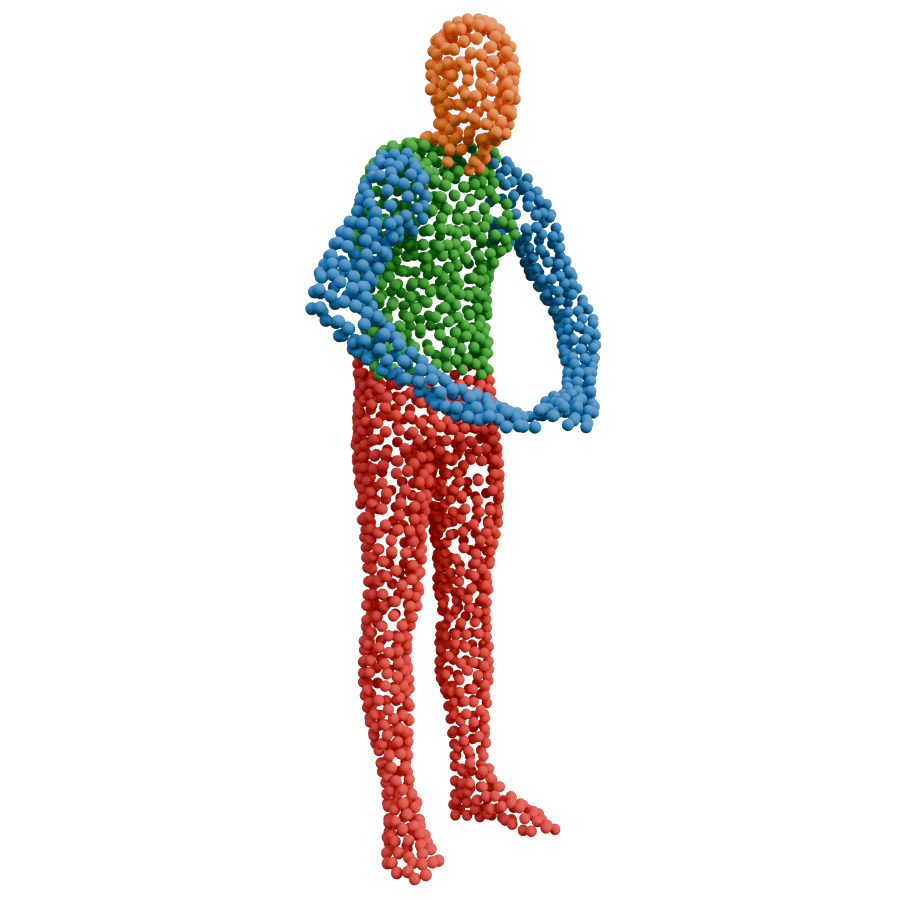
\includegraphics[width=0.30\linewidth]{figs/faust_new/tr_scan_001/GT.png} &
    
\includegraphics[width=0.30\linewidth]{figs/faust_new/tr_scan_003/GT.png} &
    
\includegraphics[width=0.30\linewidth]{figs/faust_new/tr_scan_096/GT.png} \\[4pt]

    \rowlabelnew{COPS} &
    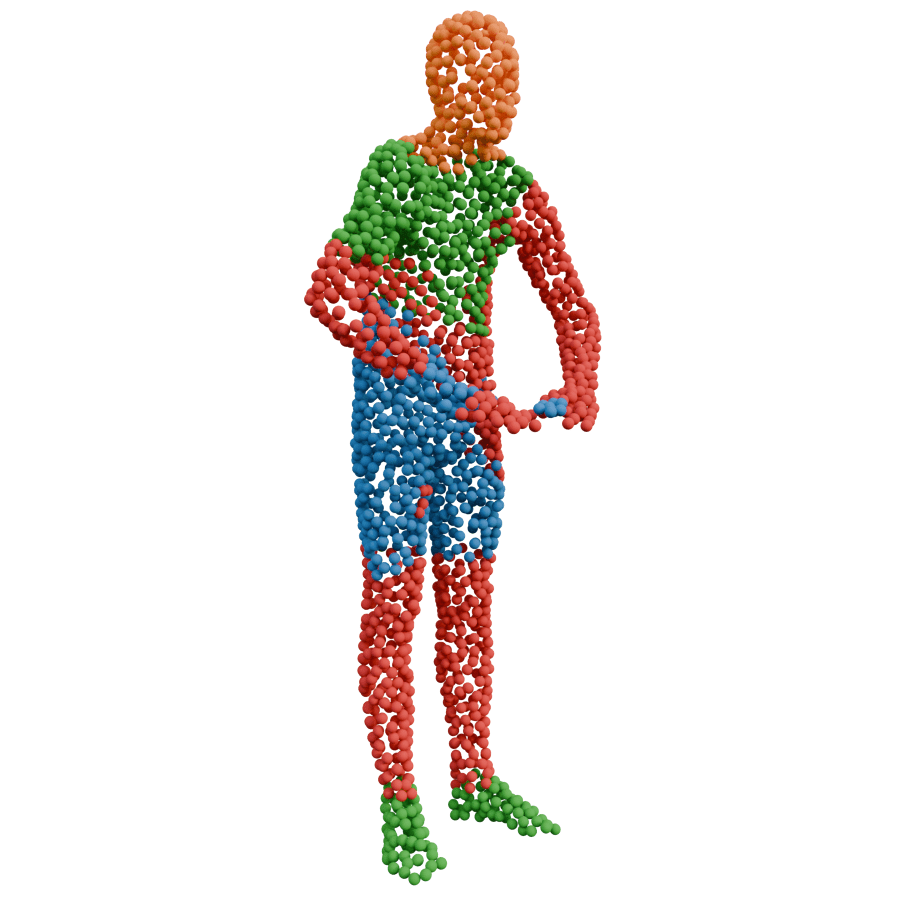
\includegraphics[width=0.30\linewidth]{figs/faust_new/tr_scan_001/COPS_HGR.png} &
    
\includegraphics[width=0.30\linewidth]{figs/faust_new/tr_scan_003/COPS_HGR.png} &
    
\includegraphics[width=0.30\linewidth]{figs/faust_new/tr_scan_096/COPS_HGR.png} \\[4pt]

    \rowlabelnew{Find3D} &
    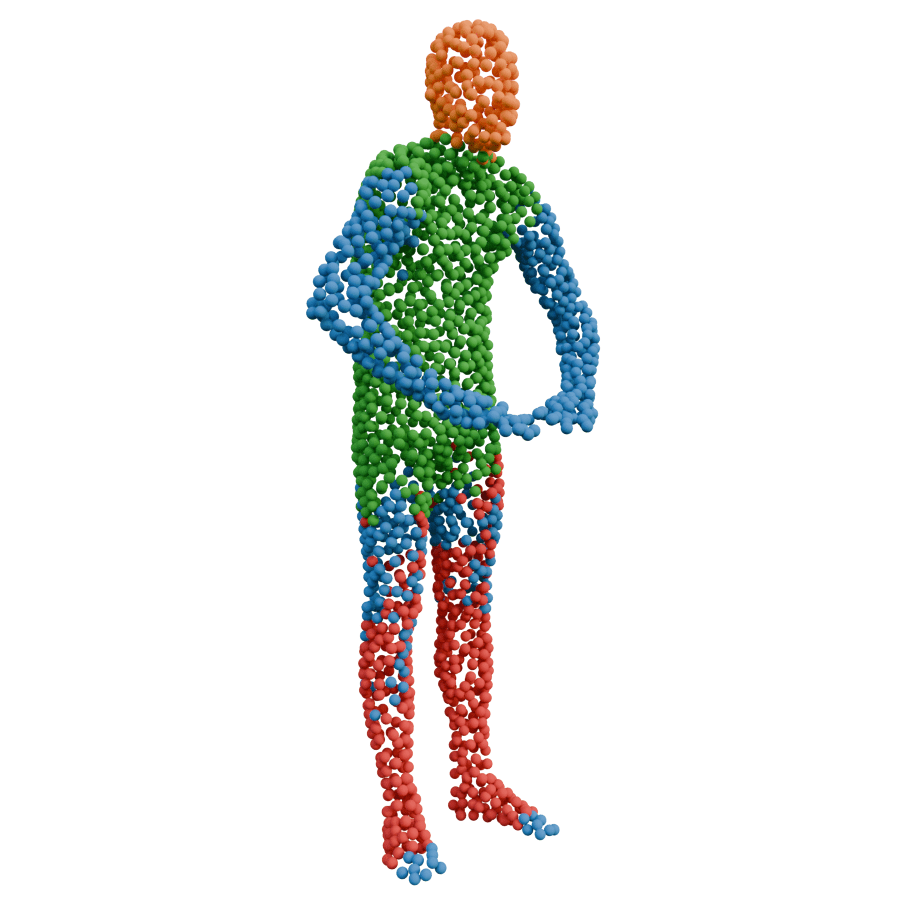
\includegraphics[width=0.30\linewidth]{figs/faust_new/tr_scan_001/Find3D.png} &
    
\includegraphics[width=0.30\linewidth]{figs/faust_new/tr_scan_003/Find3D.png} &
    
\includegraphics[width=0.30\linewidth]{figs/faust_new/tr_scan_096/Find3D.png} \\[4pt]

    \rowlabelnew{PatchAlign3D} &
    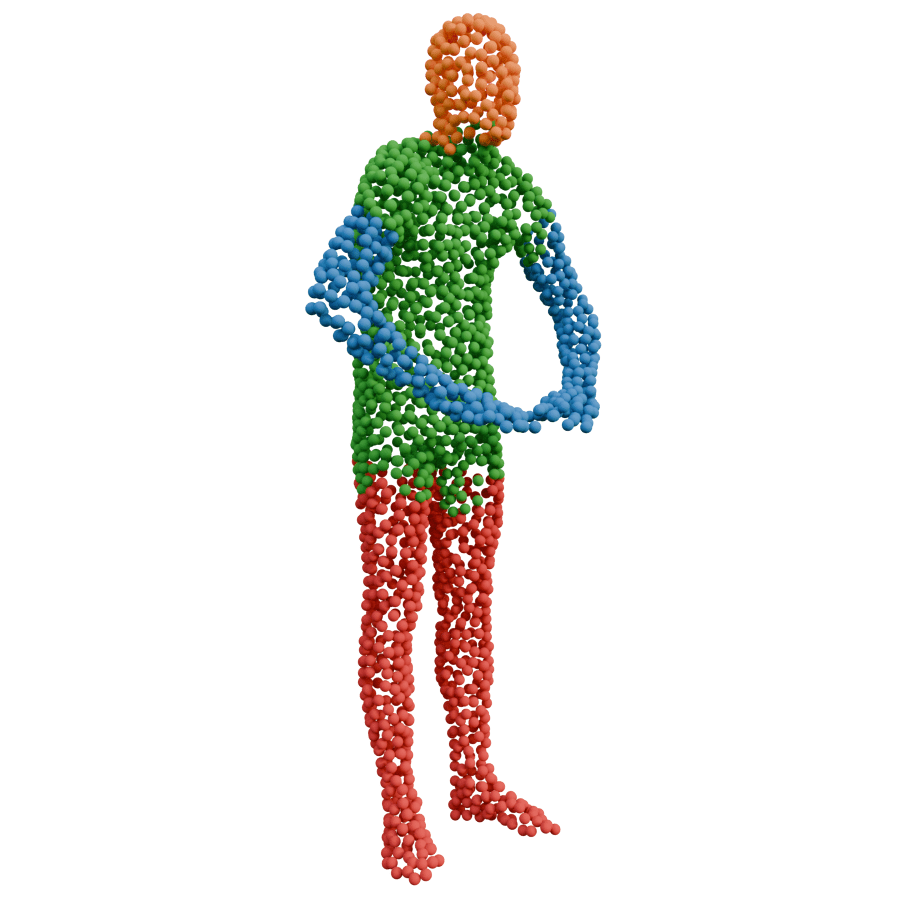
\includegraphics[width=0.30\linewidth]{figs/faust_new/tr_scan_001/PB.png} &
    
\includegraphics[width=0.30\linewidth]{figs/faust_new/tr_scan_003/PB.png} &
    
\includegraphics[width=0.30\linewidth]{figs/faust_new/tr_scan_096/PB.png} \\[2pt]

    & \multicolumn{3}{c}{\scriptsize
      \{\textcolor{blue}{arm}, \textcolor{orange}{head}, \textcolor{red}{leg}, \textcolor{darkgreen}{torso}\}} \\
\end{tabular}

\caption{\textbf{Qualitative comparison on non-rigid human shapes from FAUST \cite{bogo2014faust, abdelreheem2023satr}.}
We show ground truth and predictions from COPS \cite{garosi20253d}, Find3D \cite{ma2025find}, and PatchAlign3D across three
representative shapes (columns). The part legend below specifies the semantic labels
used for zero-shot prediction. PatchAlign3D produces cleaner segmentations than prior
methods and is less noisy than Find3D's encoder–decoder outputs.}

    \label{fig:humans_3x4}
\end{figure}


\mypara{Metrics.}
We report two aggregated segmentation metrics: mean Intersection-over-Union over instances (mIoU) and mean category-wise Intersection-over-Union (cIoU). 
In our setting, mIoU averages part-wise IoU over all test shapes, giving equal weight to each instance regardless of category frequency. 
cIoU averages IoU across object categories before aggregation, making it less sensitive to dataset imbalance. 
Both metrics capture the quality and consistency of part predictions in a zero-shot context.

\mypara{Baselines.}
We compare PatchAlign3D against both rendering-based vision–language methods and feed-forward 3D encoders.
Among rendering-based approaches, we include PointCLIPv2 \cite{zhu2022pointclip}, which leverages CLIP \cite{radford2021learning} features, and COPS \cite{garosi20253d}, which uses dense DINOv2 \cite{oquab2023dinov2} features. 
As a feed-forward baseline, we evaluate Find3D~\cite{ma2025find}, an encoder–decoder architecture trained on the same dataset as our approach and designed to produce point-level features aligned with language.
For reference, we also report the mesh-based methods SATR \cite{abdelreheem2023satr} and 3DH \cite{decatur20233d}, although they use high-resolution meshes rather than point clouds and are therefore not strictly comparable. 
Additionally, we include PartSLIP \cite{liu2023partslip} on the PartNetE benchmark, where it performs strongly, but its inference cost (several minutes per shape) makes evaluation on all benchmarks impractical. 
When baseline results were unavailable, we re-ran models using their official code. 
Finally, to avoid prompt engineering bias, we follow a unified template ("\{part\}", "a \{part\}", "\{part\} part") for all textual descriptions and re-run experiments when necessary to ensure consistency.

\mypara{Implementation settings.}
For Stage 1 distillation, we extract visual features using DINOv2 \cite{oquab2023dinov2} to remain consistent
with prior work such as COPS. We ablate alternative visual encoders in the supplementary material. For Stage 2 and inference, we employ the widely used OpenCLIP ViT-bigG-14 text encoder~\cite{radford2021learning}, following recent 3D foundation models~\cite{liu2023openshape, zhou2023uni3d}. An ablation of different text encoders is provided in the supplementary material.

Throughout both training and inference, PatchAlign3D uses only XYZ coordinates as input to point clouds of size 2048. The number of patches is fixed to 128, and each patch contains 32 points.
In contrast, several baselines (e.g., Find3D) incorporate richer input modalities such as
RGB colors and surface normals whenever available.

We train both Stage 1 and Stage 2 for 100 epochs with a batch size of 32 using the
same training set. In Stage 2, we fine-tune only the last transformer block and the
projector, leaving the remaining layers frozen. We ablate this freezing strategy in the
supplementary material. We implement the whole framework in PyTorch \cite{paszke2019pytorch}.


%, we intend to release the complete implementation.



\begin{table}[t]
\centering
\resizebox{\columnwidth}{!}{%
\begin{tabular}{l|l|c|cccc}
\hline
\textcolor{gray}{Pipeline} & Method & mIoU & Arm & Head & Leg & Torso \\ \hline
\multicolumn{7}{c}{Mesh methods} \\ \hline
\textcolor{gray}{Rendering} & 3DH~\cite{decatur20233d}  & 16.5 & 28.6 & 14.2 & 14.9 & 8.2 \\
\textcolor{gray}{Rendering} & SATR~\cite{abdelreheem2023satr}\,*  & 59.6 & 44.8 & 73.2 & 65 & 55.4 \\
% mesh & SATR & 82.5 & 85.9 & 90.6 & 85.8 & 67.6 \\ \hline
\hline
\multicolumn{7}{c}{Point-cloud methods} \\ \hline
\textcolor{gray}{Rendering} & PointCLIPv2~\cite{zhu2022pointclip}  & 13.6 & 14.0 & 15.8 & 24.1 & 0.3 \\
\textcolor{gray}{Rendering} & COPS~\cite{garosi20253d} & 30.4 & 29.8 & 33.4 & 48.2 & 10.2 \\
\textcolor{gray}{Feed-forward} & Find3D~\cite{ma2025find} & 63.2 & 59.8 & 81.0 & 59.9 & \textbf{52.0} \\
\rowcolor{OursTint}
\textcolor{gray}{Feed-forward} & PatchAlign3D & \textbf{67.8} & \textbf{68.7} & \textbf{86.4} & \textbf{65.5} & 49.7 \\ \hline
\end{tabular}%
}
\caption{\textbf{Zero-shot part segmentation results on FAUST \cite{bogo2014faust, abdelreheem2023satr}.} Our main comparison is with point-cloud methods, although we also report mesh-based approaches for completeness. *For fairness, 
the SATR input is a mesh reconstructed from a 5000-point point cloud. 
PatchAlign3D achieves the best performance and significantly surpasses rendering-based baselines.}
\label{tab:faust}
\end{table}



\subsection{Quantitative Results}

\cref{tab:shapenetpart} reports results on ShapeNetPart, where PatchAlign3D
establishes a new state of the art in open-world segmentation. Our method surpasses the strongest prior approach,
COPS, by \textbf{+31.3\%} mIoU and \textbf{+20.9\%} cIoU, and achieves
consistent gains across 15 of the 16 object categories. It also substantially
outperforms its feed-forward counterpart, Find3D, despite both methods being trained
on the same data. These results indicate that PatchAlign3D's training pipeline produces significantly stronger local representations, even though it operates on coarser patch features.
\cref{tab:faust} shows results on FAUST's non-rigid human shapes.
PatchAlign3D again outperforms existing point-cloud methods, improving over Find3D by
\textbf{+4.6\%} mIoU.
On PartNetE (\cref{tab:partnete_scanobjectnn}), we assign a
"body" label to unlabeled points since our approach relies on patch-text similarity. Despite these constraints and the dataset's
fine-grained part definitions, PatchAlign3D maintains a clear margin over previous baselines.
ScanObjectNN introduces substantial domain shift due to real-world noise and background
clutter. As shown in \cref{tab:partnete_scanobjectnn}, PatchAlign3D still achieves
the best performance, with improvements of \textbf{+3.9\%} mIoU and \textbf{+4.3\%} cIoU over
the strongest competitor.
On the Objaverse–General benchmark (\cref{tab:objaverse_general}), our
method exceeds Find3D on both seen and unseen categories, demonstrating strong
generalization under category shift. Overall, PatchAlign3D consistently outperforms 
rendering-based methods and even the best feed-forward baseline, despite being trained on
exactly the same data.

\mypara{Inference speed.}
\cref{tab:inference_speed} compares the runtime of PatchAlign3D with rendering-based and feed-forward baselines.
PatchAlign3D achieves inference speed on par with existing feed-forward models and is faster than rendering-based approaches such as COPS. This efficiency comes from our single-pass architecture and is a key step toward real-time 3D part segmentation.

\begin{table}[t]
\centering
\tiny
\resizebox{\columnwidth}{!}{%
\begin{tabular}{lll|ll}
\hline
\multirow{2}{*}{Method} 
& \multicolumn{2}{c}{PartNetE}
& \multicolumn{2}{c}{ScanObjectNN} \\[-2pt]

\cmidrule(lr){2-3}
\cmidrule(lr){4-5}

& mIoU & cIoU & mIoU & cIoU \\ \hline

PointCLIPv2~\cite{zhu2022pointclip} & 23.8    & 26.0  &   9.0   &   11.0   \\
PartSLIP~\cite{liu2023partslip}    & --    & 36.4 & --   & --   \\
COPS~\cite{garosi20253d}        & 27.0 & 29.3 &   17.7   &   20.2   \\
Find3D~\cite{ma2025find}      & 16.4 & 17.1    &  18.8    &   21.0  \\

\rowcolor{OursTint}
PatchAlign3D &   \textbf{41.4}   &   \textbf{42.2}    &  \textbf{22.7}    &    \textbf{25.3}  \\ \hline
\end{tabular}%
}
\caption{\textbf{Zero-shot shape part segmentation on PartNetE \cite{liu2023partslip} and ScanObjectNN \cite{uy2019revisiting}.} 
PointCLIPv2, COPS, and Find3D are evaluated using part labels only. 
We also include the reported PartSLIP result on PartNetE, where it performs best, 
but do not re-evaluate it on ScanObjectNN due to its high computational cost 
(about 4 minutes per shape). PatchAlign3D achieves the highest performance across both datasets.}
\label{tab:partnete_scanobjectnn}
\end{table}




\begin{table}[t]
\centering
\small
\begin{tabular}{l|c|c}
\hline
\multirow{2}{*}{Method} 
& \multicolumn{2}{c}{Objaverse–General} \\
\cmidrule(lr){2-3}
& \shortstack[c]{Seen\\\textcolor{gray}{\scriptsize mIoU}}
& \shortstack[c]{Unseen\\\textcolor{gray}{\scriptsize mIoU}} \\ \hline
Find3D~\cite{ma2025find} & 28.9 & 34.6 \\
\rowcolor{OursTint}
PatchAlign3D & \textbf{37.49} & \textbf{35.61} \\ \hline
\end{tabular}
\caption{\textbf{Zero-shot part segmentation on Objaverse–General.}
Because the official split is not provided, we define a seen/unseen split with 
14 unseen categories. PatchAlign3D achieves the best results on both splits and 
shows strong robustness to category shift.}
\label{tab:objaverse_general}
\end{table}


\subsection{Qualitative Results}

\cref{fig:qual_4x6} presents qualitative comparisons on six representative
ShapeNetPart categories. We include the strongest rendering-based (COPS) and 
feed-forward (Find3D) baselines. PatchAlign3D consistently produces sharper and more 
faithful segmentations across a wide range of geometries. Although our method operates 
on patches, the predicted part boundaries remain well aligned with the underlying 
surfaces, and the resulting segments are spatially coherent rather than fragmented. 
In contrast, Find3D often exhibits point-level noise, with neighbouring points switching 
labels abruptly.

\cref{fig:humans_3x4} shows results on FAUST's non-rigid human shapes using coarse part 
labels. Despite operating on sparse point samples, PatchAlign3D maintains high 
segmentation quality and produces markedly cleaner predictions than prior methods. 
The rendering-based COPS baseline degrades significantly under deformation, whereas 
PatchAlign3D remains stable and is less affected by pose variation.



\begin{figure}[t]
    \centering
    \setlength{\tabcolsep}{1pt}
    \renewcommand{\arraystretch}{0}

    \begin{tabular}{@{}ccc@{}}
        % ---- Row 1: Shape A ----
        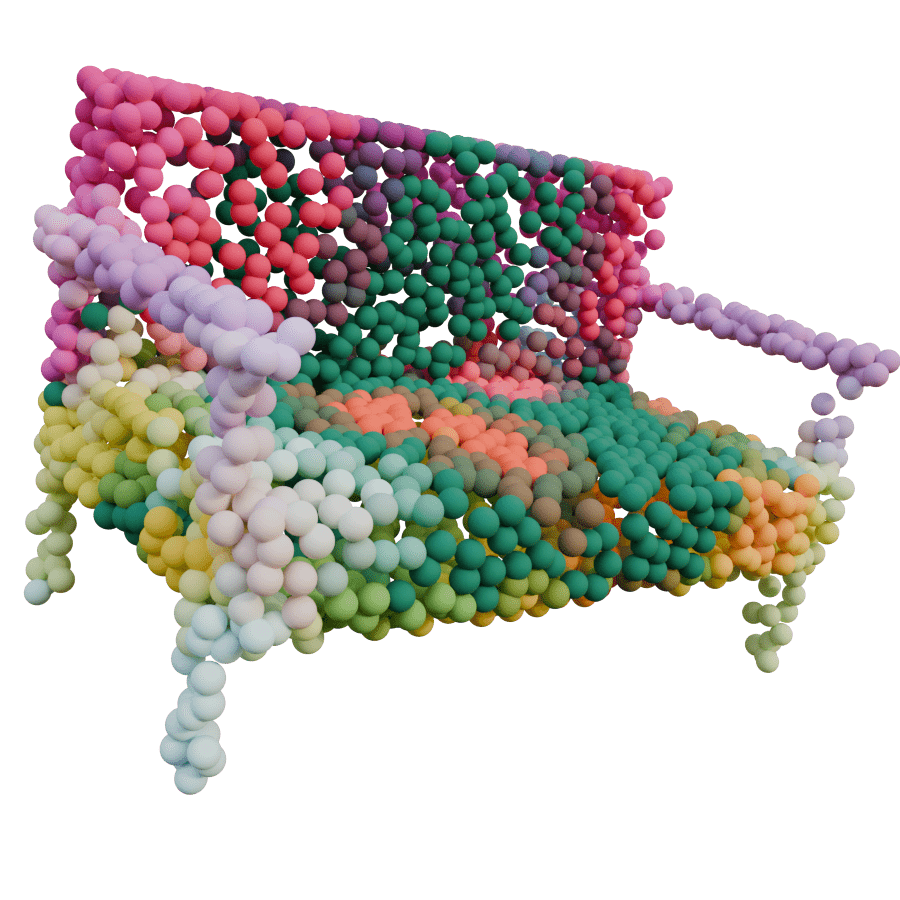
\includegraphics[width=0.31\linewidth]{figs/ablation/futon_ce316248e1994ddb9b47dfc9c2efaec3_offline_dino.png} &
        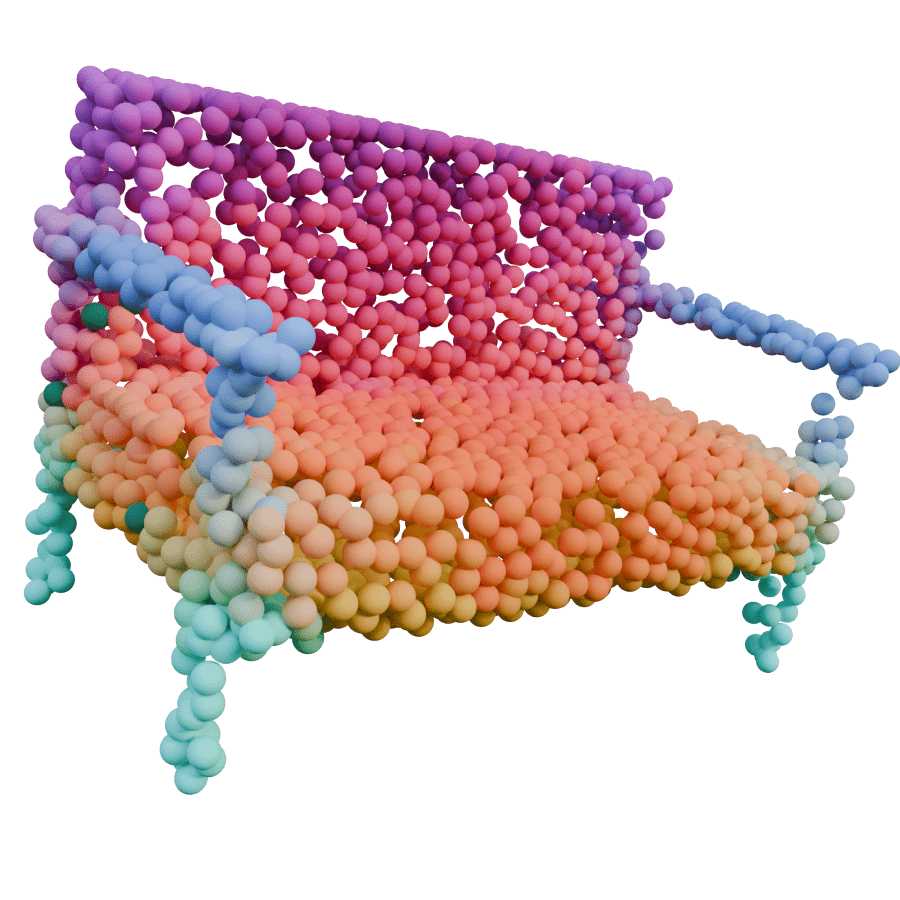
\includegraphics[width=0.31\linewidth]{figs/ablation/futon_ce316248e1994ddb9b47dfc9c2efaec3_stage1_dino.png} &
        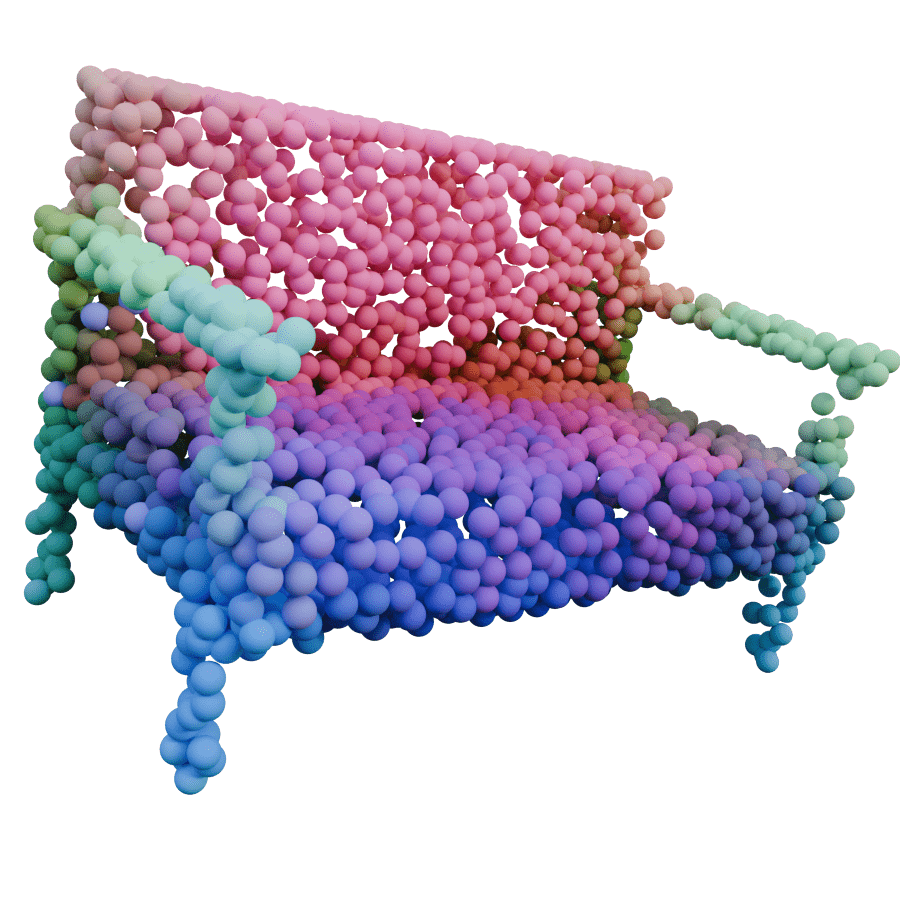
\includegraphics[width=0.31\linewidth]{figs/ablation/futon_ce316248e1994ddb9b47dfc9c2efaec3_stage2_text.png} \\[-2pt]

        % ---- Row 2: Shape B ----
        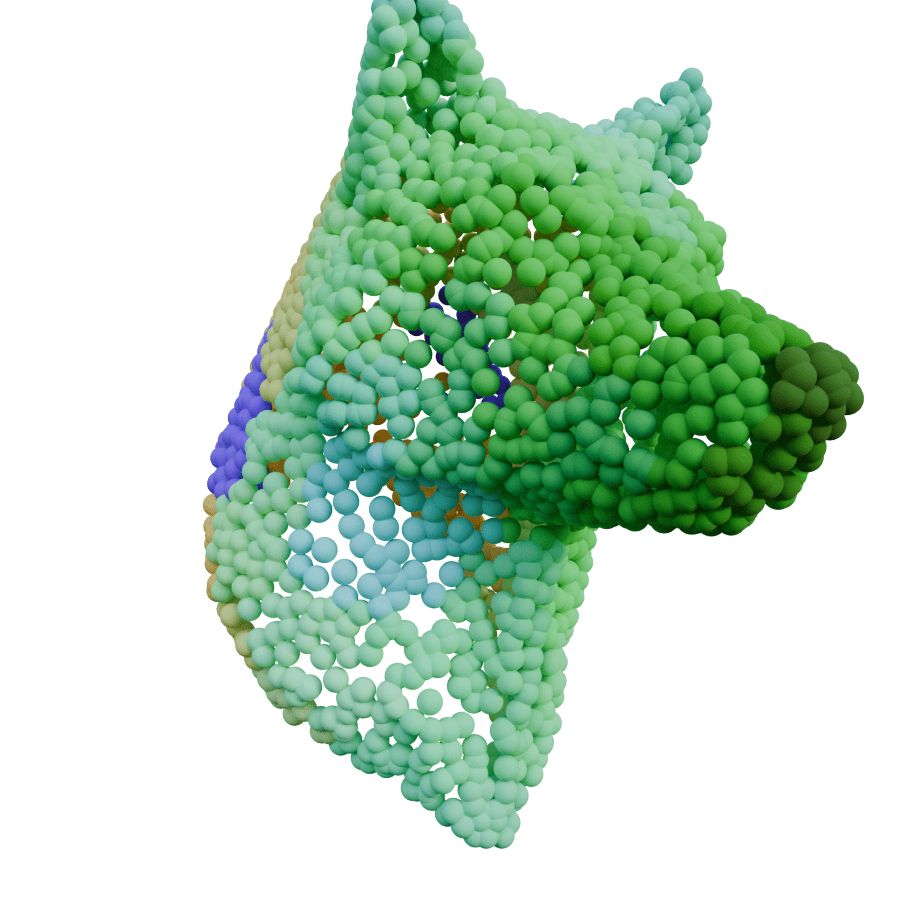
\includegraphics[width=0.31\linewidth]{figs/ablation/wolf_7298c99444704c3da07851bb28a8cf51_offline_dinov2.png} &
        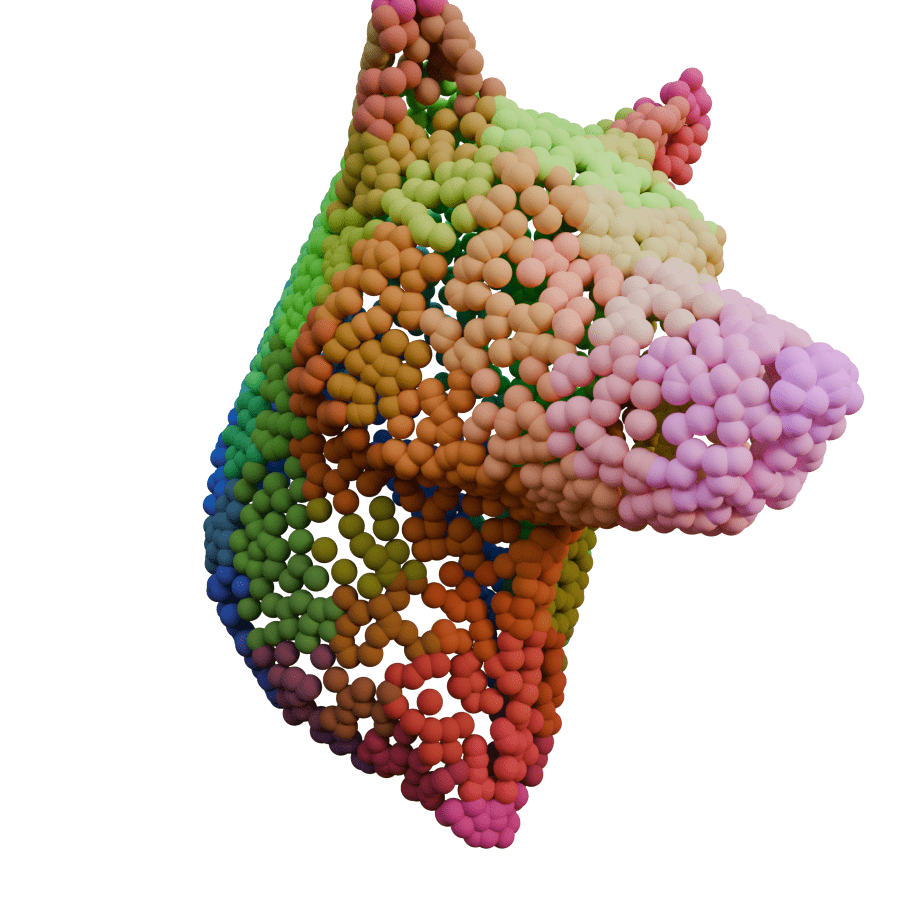
\includegraphics[width=0.31\linewidth]{figs/ablation/wolf_7298c99444704c3da07851bb28a8cf51_stage1_dinov2.png} &
        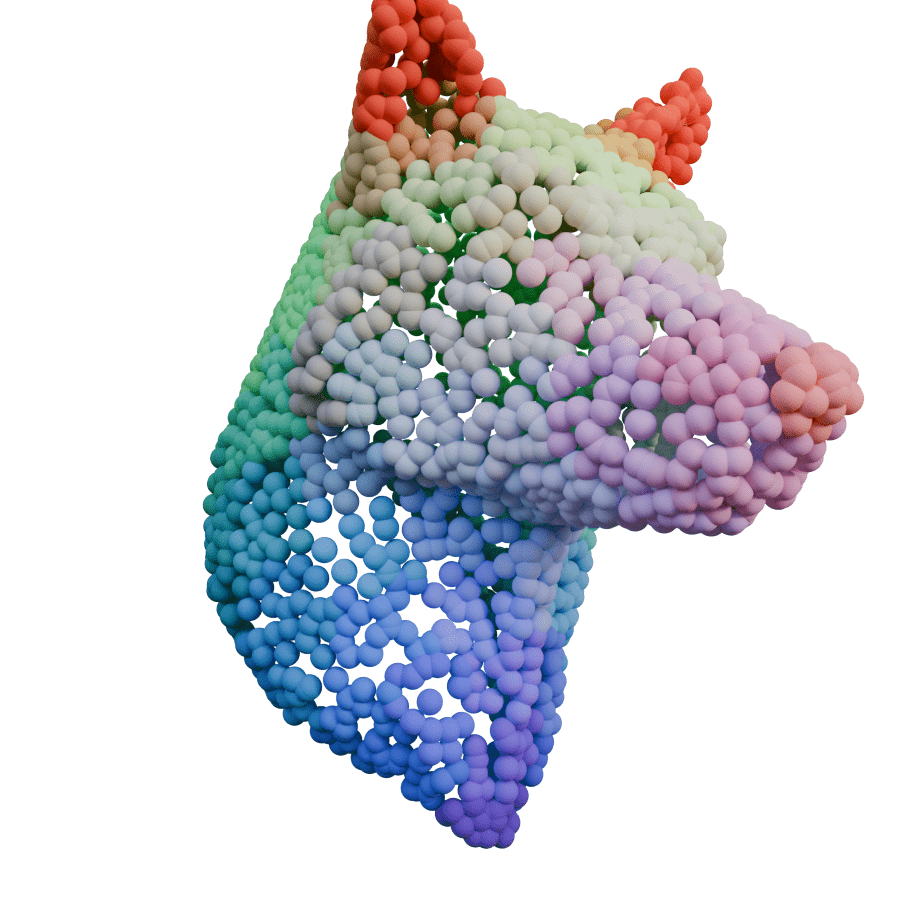
\includegraphics[width=0.31\linewidth]{figs/ablation/wolf_7298c99444704c3da07851bb28a8cf51_stage2_text.png} \\[3pt]

        % ---- Column labels (subcaptions) ----
        {\scriptsize (a) DINOv2} &
        {\scriptsize (b) Stage 1} &
        {\scriptsize (c) Stage 1 + Stage 2} \\
    \end{tabular}

    \caption{\textbf{Feature comparison across stages.}
    We visualize features from DINOv2, Stage 1, and Stage 1 + Stage 2 of our approach
    on example point clouds from the validation split of the training data.
    Stage 1 refines DINOv2 features, and Stage 2 further preserves them while assigning downstream text capabilities.}
    \label{fig:stage_features}
\end{figure}


\subsection{Ablation Study}

\mypara{Multi-stage pre-training strategy.}
\cref{tab:ablation_stage} examines the contribution of our two-stage pre-training framework. We observe that \textbf{Stage 2 alone}, which performs multi-positive contrastive alignment between patch tokens and text embeddings, already achieves state-of-the-art zero-shot performance on the ShapeNetPart segmentation benchmark. This indicates that our patch-wise contrastive formulation is sufficiently effective to learn semantically meaningful local features even without dense 2D supervision.
Nevertheless, initializing Stage 2 from the geometry-aware representations learned during \textbf{Stage 1} yields a clear improvement.

We also validate our two-stage approach by evaluating a \textbf{joint-training} variant that jointly optimizes both losses using each stage's respective projection head. This approach performs slightly worse than Stage 2 alone. We attribute this degradation to the fundamentally different nature of the two objectives: when applied concurrently, these competing signals interfere with each other. The clear gains of our two-stage design therefore, show the importance of decoupling dense feature distillation from text alignment.

\mypara{Qualitative comparison of learned features.}
\cref{fig:stage_features} visualizes the representations produced by the 2D DINOv2 backbone, our Stage 1 encoder, and the final PatchAlign3D model (Stage 1 + Stage 2). For comparison, we project each embedding space independently to RGB using PCA. DINOv2 features are lifted to the point cloud via the same multi-view back-projection used during preprocessing, whereas Stage 1 and Stage 2 features originate from patch tokens and are assigned to points through nearest-centroid propagation. While DINOv2 offers a strong initialization, its back-projected features remain noisy and exhibit inconsistencies across the surface. Stage 1 yields notably more coherent, geometry-aware patterns: different semantic regions (e.g., the seat vs. the back of a sofa, or the nose, ears, and neck of a wolf head) form clearly separated clusters. Stage 2 preserves this structural organization and further aligns language, endowing the features with open-vocabulary semantic behavior. Together, these results show that Stage 1 successfully refines dense 2D priors into stable 3D patch embeddings, and that Stage 2 enhances them with the text-driven semantics required for zero-shot part labeling. Additional qualitative comparisons are provided in the supplementary material.






\begin{table}[t]
\centering
\small
\resizebox{\columnwidth}{!}{%
\begin{tabular}{l|c|c|c}
\hline
Method & Modality & Type & Inference Time (s) \\ \hline
SATR          & Mesh & Rendering & 111 \\
COPS          & Point Cloud  & Rendering & 1.38 \\
PointCLIPv2   & Point Cloud  & Rendering & 1.20 \\
Find3D        & Point Cloud  &  Feed-forward  & \textbf{0.4} \\
\rowcolor{OursTint}
PatchAlign3D          & Point Cloud  &  Feed-forward  & \textbf{0.4} \\ \hline
\end{tabular}%
}
\caption{\textbf{Inference speed comparison.} PatchAlign3D matches the efficiency of the feed-forward approaches and is faster than rendering-based methods.}
\label{tab:inference_speed}
\end{table}


\begin{table}[t]
\centering
\small
\resizebox{0.6\columnwidth}{!}{%
\begin{tabular}{l|cc}
\hline
Configuration & mIoU & cIoU \\ \hline
Stage 2 only & 50.5 & 50.0 \\
Joint training & 50.2 & 48.6 \\
\rowcolor{OursTint}
2-Stage (PatchAlign3D) & \textbf{56.9} & \textbf{53.1} \\ \hline
\end{tabular}%
}
\caption{\textbf{Ablation on multi-stage training strategy.}
While Stage 2 alone already surpasses prior baselines, our full two-stage training
further improves performance. In contrast, jointly optimizing both stages at once
degrades pre-training.}
\label{tab:ablation_stage}
\end{table}


